\chapter{\uppercase{Technology Setup}}

A major driving principle of the presented work is that the methodology needs to be scalable. One reason for difficulties in implementing fault detection and diagnostic algorithms and other optimization methods is that there is a significant amount of initial investment necessary. This initial investment can also be cost prohibitive. 

In more complex schemes, it may be necessary to install additional sensors that are typically not available in commercial HVAC systems. Along with the sensor cost there is the cost to tie the sensors into the BAS. The updated logic will need to be coded by a controls vendor, adding more cost. On a large campus, this reprogramming can also take a significant amount of time to complete. 

Another issue is that of risk. There is risk in that if the controls do not function properly and are too complex for the current building operator, the controls cannot be easily removed and set back to default. 

\section{Proposed Setup}

In the proposed setup, the amount of change to the existing BAS is minimal. The control logic remains exactly the same. A small executable script can be installed on the BAS computer that can host code that will send https request to a remote server holding the historical data and the optimization methods. 

Before this process can begin, the sensors will need to be mapped in a way that the server can understand. 


\begin{figure}
\begin{tikzpicture}

\node (BASComputer) at (0,0) {\includegraphics[width=3cm, height=3cm]{Images/Desktop_computer_clipart_-_Yellow_theme-MPEdits.png}};

\node (Server) at (7cm, 0) {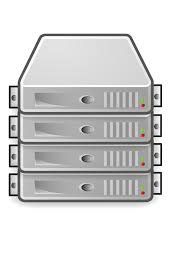
\includegraphics[width=3cm, height=3cm]{Images/serverImage.jpg}};

\draw [->, out=25, in=155, thick] (BASComputer) to node [yshift=1cm] {http request} (Server) ;

\node [above=of Server] {Web Server};

\node [right=of Server, align=left] {Historical data at \\ any syncing interval};

\end{tikzpicture}    
\caption{Diagram of networking flow.}

\end{figure}
